\documentclass[a4paper,12pt]{report}
\usepackage[utf8]{inputenc}
\usepackage[T1]{fontenc}
\usepackage[english]{babel}
\usepackage{lmodern}

%Package required to use figures
\usepackage{graphicx}

%Our chapters must be called sections
\addto\captionsenglish{\renewcommand{\chaptername}{Section}}

\begin{document}

%Code for title page
\begin{titlepage}
\centering
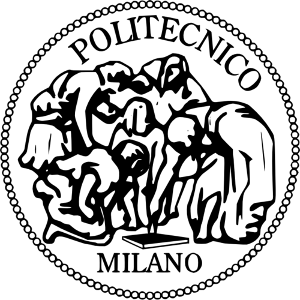
\includegraphics[width=0.20\textwidth]{./pictures/logo_poli}\par
	\vspace{1.5cm}
	{\Large {PowerEnJoy \\ 
		Software Engineering II} \par}
	\vspace{1.5cm}
	{\LARGE \textbf{Requirements Analysis and Specification Document} \par}
	\vspace{1.5cm}
	{\Large\itshape Giovanni Scotti, Marco Trabucchi\par}
	\vspace{2cm}
	\vfill
	% Bottom of the page
	{\large \today \par}
\end{titlepage}

%Make the table of contents
\tableofcontents

%INTRODUCTION
\chapter{Introduction}
\label{ch:Introduction}

\section{Purpose}
%purpose
The Design Document is intended to provide a deeper functional description of the \emph{PowerEnJoy} system-to-be by giving technical details and describing the main architectural components as well as their interfaces and their interactions. The relations among the different modules are pointed out using UML standards and other useful diagrams showing the structure of the system.

The document aims to guide the software development team to implement the architecture of the project, by providing a stable reference and a single vision of all parts of the software itself and clearly defining how they work.

\section{Scope}
The product is a digital management system to support a car-sharing service that exclusively employs electric cars.

The system consists of a back-end server application that manages rental requests remotely and three front-end applications:

\begin{itemize}
\item A web-based application to provide the final user with a friendly interface to take advantage of the services of \hbox{\emph{PowerEnJoy}};
\item An application that runs on the existing on-board computers provided on each vehicle, used to interact with the car itself, unlock it and access the GPS/sat-nav service;
\item A mobile application that allows the user to easily access the service anywhere he/she needs to.
\end{itemize}
%serve per modellare i requisiti relativi al sw del computer di bordo [vd specifiche p.3 sez.5]
%"The user is notified of the current charges through a screen on the car"

The system is intended for only one type of user: drivers, who should be allowed to register and access the system via username and password, in order to make the renting and payment processes easier and quicker to carry out. Moreover, the system aids the users by locating nearby available vehicles and keeps track of the distance driven, all while notifying them about the amount of money they are being charged. Predefined safe parking areas are signaled by an on-board computer.

Lastly, the system aims to motivate drivers to maintain a virtuous behavior providing discounts when it detects signs of responsible and ecologic actions.


\section{Definitions, Acronyms and Abbreviations}
\begin{description}
\item[RASD:] Requirements Analysis and Specification Document.
\item[System:] The software system-to-be, in all of its entirety.
\item[Driver:] See \textbf{User}.
\item[User:] Any person subscribed to the service who rents a car using \hbox{\emph{PowerEnJoy}}.
\end{description}



\section{Definitions, Acronyms and Abbreviations}
This document follows the guidelines provided by ISO/IEC/IEEE 29148:2011~\cite{ieee-29148} and IEEE 830-1998~\cite{ieee-830} respectively related to the requirements engineering for systems and software products and the recommended practice for software requirements specifications.

Moreover it is strictly based on the specifications concerning the RASD assignment~\cite{se-assignments} for the Software Engineering II project, part of the course held by professors Luca Mottola and Elisabetta Di Nitto at the Politecnico di Milano, A.Y. 2016/17.

\end{document}